% ==============================================================================
% CAPÍTULO 1: PLAN DE ADMINISTRACIÓN DE PROYECTOS DE SOFTWARE (Orquestador del Capítulo)
% ==============================================================================
% Estructura alineada con el índice de referencia (Documento.pdf, cap. 1):
%   1.1 Antecedentes · 1.2 Descripción del problema · 1.3 Desafíos · 1.4 Métricas
%   1.5 Estimaciones · 1.6 Análisis de riesgo · 1.7 Tabla de recursos
%   1.8 Planificación de tiempo · 1.9 Organización interna
%   1.10 Seguimiento y control · 1.11 Tecnologías · 1.12 Anexos
% Las secciones 1.1, 1.2, 1.7 y 1.8 reutilizan el contenido de secciones/02_capitulo1_perfil/
% (el título de 1.2, 1.7 y 1.8 se escribe aquí; el cuerpo viene de los archivos *_cuerpo.tex).
\preportadacapitulo{1}{Plan de Administración de Proyectos de Software}

\newpage
\section{Capítulo 1: Plan de Administración de Proyectos de Software}\label{cap:paps}

% ------------------------------------------------------------------------------
% 1. ANTECEDENTES
% ------------------------------------------------------------------------------
\subsection{\pfxperfil 1. Antecedentes}\label{sec:antecedentes}
% [INSTRUCCIÓN]: Describir los antecedentes históricos, institucionales y
% operativos del comedor universitario o del sistema previo de postulación.
% Incluir referencias a proyectos similares o evoluciones institucionales.

El comedor universitario constituye un servicio esencial dentro del bienestar estudiantil en las instituciones de educación superior, pues garantiza que los estudiantes —especialmente aquellos con severas limitaciones socioeconómicas— accedan a una alimentación adecuada, equilibrada y asequible (cubriendo prestaciones de desayuno, almuerzo y cena). Históricamente, estos programas de asistencia social han cumplido un rol determinante al contribuir a la permanencia estudiantil, disminuir la deserción por vulnerabilidad económica y favorecer un rendimiento académico óptimo.

En el modelo institucional actual, la administración del servicio de alimentación se encuentra tercerizada a una empresa privada. Bajo este esquema de convenio corporativo, la empresa concesionaria asume la operación del comedor a cambio de la libertad de comercializar platos a la comunidad universitaria regular (estudiantes no becados, docentes y administrativos), percibiendo ingresos directos por dichas ventas. A su vez, como parte del acuerdo institucional, la empresa privada asume compromisos de retribución como la atención alimentaria de comitivas, eventos oficiales e invitados especiales de la universidad.

Sin embargo, mientras que la logística operativa de la cocina y el expendio directo de alimentos recae en el sector privado, la responsabilidad de evaluar, seleccionar y adjudicar el beneficio de la beca comedor sigue siendo exclusivamente institucional. Tradicionalmente, este proceso de postulación se realiza de forma manual mediante la recepción masiva de documentación en físico (folders), lo cual genera una brecha crítica entre la alta demanda estudiantil y la capacidad operativa de revisión por parte de la administración universitaria.


\subsection{1.2. Descripción del problema}\label{sec:descripcion_problema_paps}
\subsubsection{\pfxperfil 2.1. Situación problemática}\label{sec:situacion_problematica}
% [INSTRUCCIÓN]: Detallar las deficiencias, demoras, errores manuales y cuellos
% de botella del proceso actual de evaluación y selección.

Actualmente, el proceso de postulación y asignación de la beca comedor se enfrenta a una ineficiencia estructural severa debido a la falta de herramientas tecnológicas automatizadas de filtrado y evaluación.

En cada gestión académica, la universidad recibe una cifra masiva que ronda las 20,000 carpetas (folders) de postulantes. Dada la escala de esta demanda y los limitados recursos humanos administrativos para la revisión física de documentos, no se logra auditar ni el 50\% de las solicitudes presentadas, alcanzando a revisar únicamente un aproximado de 8,000 carpetas. Considerando que la disponibilidad de becas es altamente restrictiva (cubriendo únicamente a cerca de 900 beneficiarios, cifra que fluctúa según el presupuesto de cada gestión), el método actual de revisión manual introduce serios sesgos e injusticias operativas:

\begin{itemize}
    \item \textbf{Revisión por orden de llegada o al azar:} Al no poder revisar la totalidad de las 20,000 carpetas, miles de postulantes en situación de extrema vulnerabilidad quedan automáticamente descalificados o ignorados simplemente porque su expediente no llegó a ser abierto.

    \item \textbf{Carga burocrática y desperdicio de recursos:} La manipulación, archivo y almacenamiento de miles de folders físicos genera un costo logístico elevado, consumo masivo de papel y el riesgo constante de extravío de documentos socioeconómicos sensibles.

    \item \textbf{Falta de transparencia y lentitud:} La verificación manual de requisitos (ingresos familiares, patrimonio, procedencia, rendimiento académico) es propensa a errores humanos, duplicidades y posibles manipulaciones, ralentizando la publicación de las listas definitivas de beneficiarios.
\end{itemize}

Por lo tanto, la problemática central reside en la incapacidad del sistema manual actual para garantizar que las limitadas becas disponibles se otorguen objetivamente a los estudiantes que presentan el mayor grado de necesidad socioeconómica, derivado de un cuello de botella en la fase de revisión de documentos. La Figura~\ref{fig:distribucion_carpetas} ilustra la distribución porcentual de las solicitudes según su destino en el proceso actual.

% ---- FIGURA: Distribución de carpetas (APA 7) --------------------------------
\begin{figure}[htbp]
\caption{Distribución porcentual de las solicitudes de beca comedor por destino en el proceso manual de revisión}
\label{fig:distribucion_carpetas}
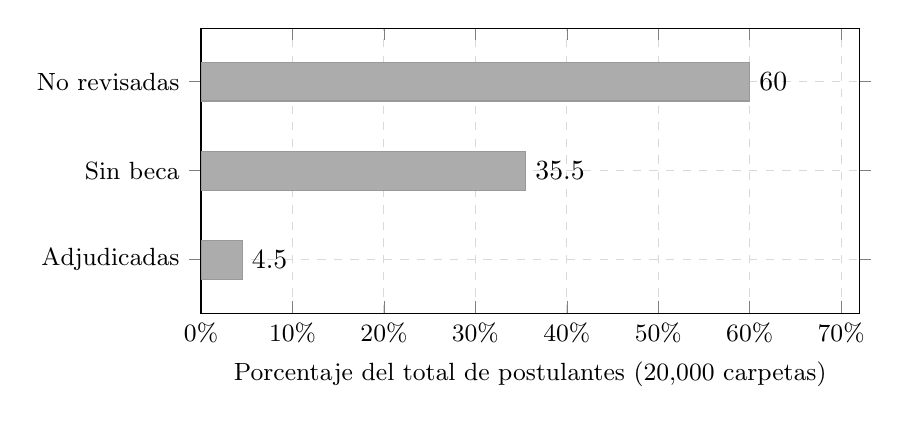
\begin{tikzpicture}
\begin{axis}[
    xbar,
    width=0.82\linewidth,
    height=5.2cm,
    bar width=14pt,
    xmin=0, xmax=72,
    ymin=0.4, ymax=3.6,
    xtick={0,10,20,30,40,50,60,70},
    xticklabel={\pgfmathprintnumber{\tick}\%},
    xlabel={Porcentaje del total de postulantes (20{,}000 carpetas)},
    ytick={1,2,3},
    yticklabels={Adjudicadas, Sin beca, No revisadas},
    nodes near coords,
    nodes near coords align={horizontal},
    grid=major,
    grid style={dashed, gray!30},
    tick label style={font=\small},
    label style={font=\small},
]
\addplot[
    fill=gray!65,
    draw=gray!80,
] coordinates {
    (4.5,  1)
    (35.5, 2)
    (60,   3)
};
\end{axis}
\end{tikzpicture}

\smallskip
\noindent\raggedright\textit{Nota.} Elaboración propia en base a datos institucionales de la gestión académica vigente. De las 20,000 carpetas recibidas, aproximadamente 12,000 (60\%) no llegan a ser revisadas; 7,100 (35,5\%) son revisadas pero no obtienen el beneficio; y solo 900 (4,5\%) corresponden a becas efectivamente adjudicadas.
\end{figure}
% ------------------------------------------------------------------------------



\subsubsection{\pfxperfil 2.2. Situación deseada}\label{sec:situacion_deseada}
% [INSTRUCCIÓN]: Explicar el estado ideal esperado tras la implantación de la solución:
% agilidad, transparencia, trazabilidad y automatización.

La situación deseada contempla la transformación digital del proceso de selección mediante la implementación de un Sistema Web y Móvil Inteligente para la Postulación y Precalificación Automática de Becas Alimentarias. Bajo este nuevo esquema:

\begin{itemize}
    \item \textbf{Digitalización y Autogestión:} Los estudiantes realizarán su postulación 100\% en línea, adjuntando la documentación requerida en formato digital.

    \item \textbf{Precalificación y Puntuación Autómata (Algoritmo de Priorización):} El sistema implementará un algoritmo de evaluación socioeconómica ponderada que analizará automáticamente los datos ingresados por el postulante (ingresos, dependientes, procedencia, estado de vulnerabilidad, promedio académico, etc.), asignando una puntuación de riesgo o necesidad en tiempo real.

    \item \textbf{Optimización de la Revisión Administrativa:} En lugar de revisar 8,000 carpetas al azar de un universo de 20,000, el personal administrativo enfocará su trabajo de validación física y auditoría exclusivamente en las carpetas con los puntajes de precalificación más altos. Esto asegura matemáticamente que los expedientes revisados correspondan a los mejores y más necesitados candidatos para adjudicarse los 900 cupos disponibles.

    \item \textbf{Transparencia y Trazabilidad:} Los estudiantes podrán consultar en tiempo real el estado de su solicitud y la puntuación obtenida, reduciendo la incertidumbre y garantizando la equidad del proceso.
\end{itemize}

\subsubsection{\pfxperfil 2.3. Objeto de la investigación}\label{sec:objeto_investigacion}
% [INSTRUCCIÓN]: Delimitar con precisión el objeto de estudio/investigación
% (p. ej., el proceso de gestión, preselección y asignación de beneficios).

El objeto de la investigación es diseñar e implementar un sistema de información para la gestión de postulaciones y precalificación automatizada de becas alimentarias, orientado a la digitalización del expediente socioeconómico estudiantil y a la optimización del proceso de selección de beneficiarios en el comedor universitario. La Figura~\ref{fig:objeto_investigacion} muestra el objeto de estudio: el proceso mediante el cual las solicitudes de los postulantes son recibidas, preseleccionadas con apoyo de Inteligencia Artificial, auditadas por la DUBSS y convertidas en becas adjudicadas, junto con la información que el sistema entrega a las autoridades.

\begin{figure}[H]
\caption{Objeto de la investigación: proceso de postulación y preselección de la Beca Comedor apoyado por el sistema de información}
\label{fig:objeto_investigacion}
\centering
\begin{tikzpicture}[
    node distance=0.55cm and 0.7cm,
    box/.style={draw, rounded corners=2pt, align=center, minimum height=2.3cm, text width=2.6cm, inner sep=2pt, font=\footnotesize\linespread{1}\selectfont},
    sys/.style={box, fill=gray!15},
    arr/.style={-{Stealth[length=2.5mm]}, thick}
]
\node[box] (post) {Postulantes\\(estudiantes)};
\node[sys, right=of post] (form) {Postulación en línea\\(web y móvil)};
\node[sys, right=of form] (ia) {Preselección con IA\\(puntaje de vulnerabilidad)};
\node[box, below=0.9cm of ia] (aud) {Auditoría y adjudicación\\(personal DUBSS)};
\node[box, left=of aud] (beca) {Beca Comedor\\(\textasciitilde900 beneficiarios)};
\node[sys, left=of beca] (bi) {Reportes BI\\(autoridades)};
\draw[arr] (post) -- (form);
\draw[arr] (form) -- (ia);
\draw[arr] (ia) -- (aud);
\draw[arr] (aud) -- (beca);
\draw[arr] (beca) -- (bi);
\end{tikzpicture}

\smallskip
\noindent\raggedright\textit{Nota.} Elaboración propia. Los bloques sombreados corresponden a los componentes que se desarrollan en el proyecto.
\end{figure}

\begin{figure}[H]
\caption{Evolución de la selección de la Beca Comedor: de la revisión manual a la precalificación automática}
\label{fig:evolucion_seleccion}
\centering
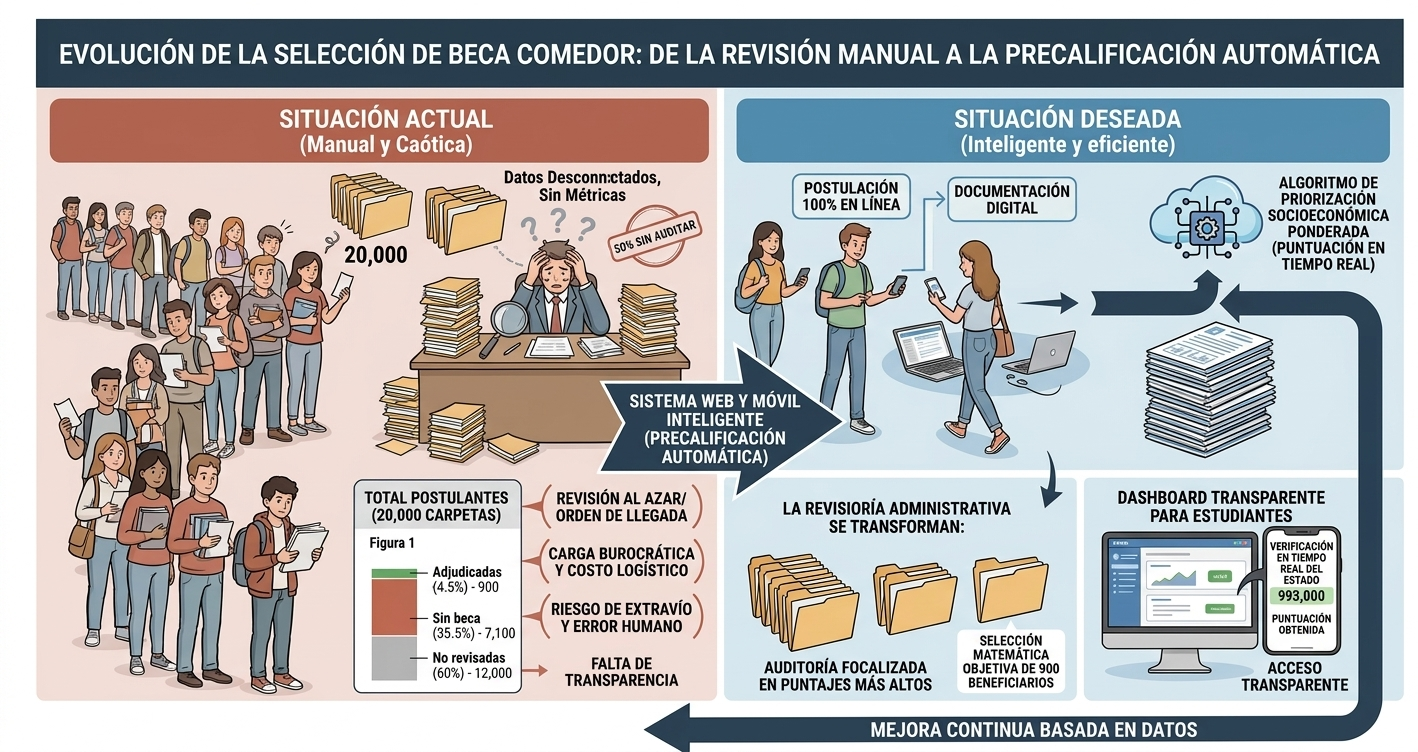
\includegraphics[width=\textwidth]{images/021_Objeto_Investigacion.jpg}

\smallskip
\noindent\raggedright\textit{Nota.} Elaboración propia.
\end{figure}


% ==============================================================================
% 1.3 DESAFÍOS DE LA INGENIERÍA DE SOFTWARE
% ==============================================================================
\subsection{1.3. Desafíos de la ingeniería de software}

\subsubsection{1.3.1. Calidad}

% [PENDIENTE]: Redactar "Calidad" (cómo el proyecto aborda la calidad: IEEE 830, UML, pruebas; vincular con el SQAP del Capítulo 2).

\subsubsection{1.3.2. Productividad}

% [PENDIENTE]: Redactar "Productividad" (equipo de 2 integrantes, reparto por paquetes, herramientas).

\subsubsection{1.3.3. Innovación}

% [PENDIENTE]: Redactar "Innovación" (precalificación con IA y reportes BI aplicados a la Beca Comedor).


% ==============================================================================
% 1.4 MÉTRICAS (sobre tres software de referencia)
% ==============================================================================
% [PENDIENTE: DEFINIR CON EL EQUIPO] Los tres software de referencia. Cada uno lleva las
% mismas cinco subsecciones; las líneas de código se miden con cloc sobre el repositorio
% real (no se inventan cifras). Reemplazar «Software de referencia N» por el nombre elegido.
\subsection{1.4. Métricas}

% ---------------------------------------------------------------- Software 1
\subsubsection{1.4.1. Software de referencia 1}

\paragraph{1.4.1.1. Funcionalidades importantes.}

% [PENDIENTE]: Descripción general, repositorio, licencia y funcionalidades del software 1.

\paragraph{1.4.1.2. Captura de interfaces.}

% [PENDIENTE]: Capturas de pantalla del software 1.

\paragraph{1.4.1.3. Características del desarrollador.}

% [PENDIENTE]: Conteo de líneas de código (cloc) del software 1.

\paragraph{1.4.1.4. Métrica orientada al tamaño.}

% [PENDIENTE]: Tabla KLDC, costo, tiempo, esfuerzo, gente, calidad y productividad del software 1.

\paragraph{1.4.1.5. Aplicación de las métricas orientada a la función.}

% [PENDIENTE]: Puntos de función del software 1 (conteo, 14 factores Fi y PF final).

% ---------------------------------------------------------------- Software 2
\subsubsection{1.4.2. Software de referencia 2}

\paragraph{1.4.2.1. Funcionalidades importantes.}

% [PENDIENTE]: Ver 1.4.1.1.

\paragraph{1.4.2.2. Captura de interfaces.}

% [PENDIENTE]: Ver 1.4.1.2.

\paragraph{1.4.2.3. Características del desarrollador.}

% [PENDIENTE]: Ver 1.4.1.3.

\paragraph{1.4.2.4. Métrica orientada al tamaño.}

% [PENDIENTE]: Ver 1.4.1.4.

\paragraph{1.4.2.5. Aplicación de las métricas orientada a la función.}

% [PENDIENTE]: Ver 1.4.1.5.

% ---------------------------------------------------------------- Software 3
\subsubsection{1.4.3. Software de referencia 3}

\paragraph{1.4.3.1. Funcionalidades importantes.}

% [PENDIENTE]: Ver 1.4.1.1.

\paragraph{1.4.3.2. Captura de interfaces.}

% [PENDIENTE]: Ver 1.4.1.2.

\paragraph{1.4.3.3. Características del desarrollador.}

% [PENDIENTE]: Ver 1.4.1.3.

\paragraph{1.4.3.4. Métrica orientada al tamaño.}

% [PENDIENTE]: Ver 1.4.1.4.

\paragraph{1.4.3.5. Aplicación de las métricas orientada a la función.}

% [PENDIENTE]: Ver 1.4.1.5.


% ==============================================================================
% 1.5 ESTIMACIONES
% ==============================================================================
\subsection{1.5. Estimaciones}

\subsubsection{1.5.1. Dimensiones del proyecto}

\paragraph{1.5.1.1. Tamaño.}

% [PENDIENTE]: Redactar "Tamaño" (26 casos de uso en 6 paquetes; puntos por CU de casos_de_uso_filtrados.md / plan_desarrollo_tareas.md).

\paragraph{1.5.1.2. Complejidad.}

% [PENDIENTE]: Redactar "Complejidad".

\paragraph{1.5.1.3. Estructuración del cliente.}

% [PENDIENTE]: Redactar "Estructuración del cliente".

\subsubsection{1.5.2. Ámbito del proyecto}

\paragraph{1.5.2.1. Objetivos del proyecto.}

Desarrollar un Sistema de Información Web y Móvil para la Postulación y Preselección Automatizada de la Beca Comedor mediante Inteligencia Artificial, con Reportes de Business Intelligence para la Dirección Universitaria de Bienestar Social y Salud (DUBSS) de la Universidad Autónoma Gabriel René Moreno, que permita automatizar la postulación en línea, precalificar algorítmicamente la vulnerabilidad socioeconómica de los estudiantes, gestionar la asistencia física/digital y proveer dashboards analíticos y proyecciones predictivas que apoyen la toma de decisiones institucionales y auditorías.


\paragraph{1.5.2.2. Objetivos específicos.}

\begin{itemize}
    \item Capturar los requisitos funcionales y no funcionales del proceso de postulación y adjudicación de la Beca Comedor mediante entrevistas con el personal de la DUBSS, y especificarlos según el estándar IEEE 830.

    \item Analizar los procesos del sistema modelando los casos de uso y el dominio mediante UML, y definir las reglas de negocio de la preselección.

    \item Diseñar la arquitectura general del sistema web y móvil, y las interfaces de usuario para cada tipo de usuario.

    \item Implementar los módulos del sistema web y móvil, integrando la preselección automatizada con inteligencia artificial y los reportes de Business Intelligence.

    \item Realizar pruebas de caja negra y de caja blanca que verifiquen el cumplimiento de los requisitos especificados.
\end{itemize}


\paragraph{1.5.2.3. Requerimientos principales.}

Los requerimientos del sistema se especifican en las secciones 3.2.1 a 3.2.3 (Especificación de Requisitos de Software según la IEEE 830) del Capítulo 3, y los casos de uso que los implementan, en las secciones 3.2.4 a 3.2.8.

\paragraph{1.5.2.4. Rendimiento.}

% [PENDIENTE]: Redactar "Rendimiento" (RNF: carga <= 3 s, puntaje individual <= 5 s, 20,000 postulaciones por gestión, >= 50 administrativos concurrentes).

\paragraph{1.5.2.5. Fiabilidad.}

% [PENDIENTE]: Redactar "Fiabilidad" (disponibilidad >= 99 % en periodos de postulación y evaluación; idempotencia, RNF-03).

\paragraph{1.5.2.6. Restricciones.}

\begin{itemize}
    \item \textbf{Requisito de Auditoría Física (Restricción Normativa):} El sistema no elimina por completo el uso de papel en la fase de asistencia diaria, debido a la exigencia reglamentaria de los organismos auditores que requieren carpetas físicas con fotocopia de carnet y firma manuscrita para validar la entrega del alimento a cada becado. El software actuará como un medio de control, validación y archivo digitalizador complementario.

    \item \textbf{Operación Interna de la Cocina:} El sistema no gestiona el control de inventarios de insumos, compras de materia prima ni la contabilidad interna de la empresa privada concesionaria del comedor.

    \item \textbf{Comercialización a No Becados:} La venta de almuerzos y platos a estudiantes regulares no becados y personal universitario queda fuera del alcance del sistema, correspondiendo a la gestión propia de la empresa privada.

    \item \textbf{Dependencia de Conectividad:} La carga de expedientes y la sincronización de asistencias requieren conexión a Internet activa.

    \item \textbf{Límites de Verificación Automática:} El sistema realiza una precalificación algorítmica basada en la información declarada y digitalizada; sin embargo, la verificación presencial o visitas domiciliarias mantendrán el criterio operativo del personal de Trabajo Social.
\end{itemize}


\paragraph{1.5.2.7. Infraestructura externa.}

% [PENDIENTE]: Redactar "Infraestructura externa" (Firebase Auth, FCM y Storage; AWS; módulo de IA en Python).

\subsubsection{1.5.3. Estimaciones para el proyecto}

\paragraph{1.5.3.1. Valor esperado.}

% [PENDIENTE]: Redactar "Valor esperado".

\paragraph{1.5.3.2. COCOMO II.}

% [PENDIENTE]: Redactar "COCOMO II".

\paragraph{1.5.3.3. La ecuación del software.}

% [PENDIENTE]: Redactar "La ecuación del software".

\paragraph{1.5.3.4. Planning póker.}

% [PENDIENTE]: Redactar "Planning póker" (sobre casos de uso, no historias de usuario).


% ==============================================================================
% 1.6 ANÁLISIS DE RIESGO
% ==============================================================================
\subsection{1.6. Análisis de riesgo}

\subsubsection{1.6.1. Identificación de riesgo}

% [PENDIENTE]: Redactar "Identificación de riesgo". Los riesgos propios del proyecto se confirman con el equipo.

\subsubsection{1.6.2. Probabilidad de presencia de riesgo}

% [PENDIENTE]: Redactar "Probabilidad de presencia de riesgo" (tabla riesgo, probabilidad, impacto, reducir probabilidad, reducir impacto).


\subsection{1.7. Tabla de recursos}\label{sec:tabla_recursos_paps}
\subsubsection{\pfxperfil 7.1. Software y herramientas}\label{sec:recursos_software}
% [INSTRUCCIÓN]: Lenguajes, frameworks, bases de datos, servidores, IDEs.

\begin{table}[H]
\caption{Software y herramientas utilizados para el desarrollo del proyecto}
\label{tab:software_herramientas}
\begin{threeparttable}
\begin{tabular}{>{\raggedright\arraybackslash}p{4.5cm} >{\raggedright\arraybackslash}p{8.5cm}}
\toprule
Software y herramienta & Descripción \\
\midrule
Windows 11 & Sistema operativo utilizado como plataforma base en los equipos de desarrollo. \\
Visual Studio Code & Editor de código fuente donde se escribe y depura el código del sistema. \\
Bruno / Postman & Herramientas para diseñar, documentar y probar las API del sistema. \\
GitHub & Plataforma para el control de versiones y el trabajo colaborativo del código fuente. \\
Enterprise Architect & Herramienta de modelado UML para elaborar los diagramas del sistema. \\
Jira & Plataforma de gestión de proyectos para organizar y dar seguimiento a las tareas de desarrollo. \\
Docker & Plataforma de contenedores para estandarizar los entornos de desarrollo y despliegue. \\
\bottomrule
\end{tabular}
\begin{tablenotes}
\item \textit{Nota.} Elaboración propia.
\end{tablenotes}
\end{threeparttable}
\end{table}

\subsubsection{\pfxperfil 7.2. Equipos y hardware}\label{sec:recursos_hardware}
% [INSTRUCCIÓN]: Computadoras, servidores, dispositivos IoT, dispositivos móviles, entre otros.

\begin{table}[H]
\caption{Equipos y hardware requeridos para el desarrollo del proyecto}
\label{tab:equipos_hardware}
\begin{threeparttable}
\begin{tabular}{>{\raggedright\arraybackslash}p{4.5cm} >{\raggedright\arraybackslash}p{8.5cm}}
\toprule
Recurso / equipo & Especificación y uso \\
\midrule
PC de desarrollo 1 & Computadora con procesador AMD Ryzen 7 8700G y 16 GB de RAM, utilizada para el desarrollo del sistema. \\
PC de desarrollo 2 & Computadora con procesador AMD Ryzen 7 5600G y 16 GB de RAM, utilizada para el desarrollo del sistema. \\
Redmi Note 14 Pro & Dispositivo móvil Android utilizado para probar la aplicación móvil. \\
Honor X8 & Dispositivo móvil Android utilizado para probar la aplicación móvil. \\
Servidor AWS & Servidor en la nube de Amazon Web Services utilizado para el despliegue de la aplicación y la base de datos. \\
\bottomrule
\end{tabular}
\begin{tablenotes}
\item \textit{Nota.} Elaboración propia.
\end{tablenotes}
\end{threeparttable}
\end{table}

\subsubsection{\pfxperfil 7.3. Presupuesto estimado}\label{sec:presupuesto_estimado}
% [INSTRUCCIÓN]: Costos de licencias, servidores en la nube, adquisición de equipos o contratación.

El presupuesto estimado del proyecto contempla los costos de hardware, software, recursos humanos, infraestructura y logística durante el periodo comprendido entre el 24 de agosto de 2026 y el 30 de noviembre de 2026 (3 meses). Sobre los equipos de hardware se aplica una depreciación del 10\% por su uso durante el desarrollo. Las Tablas~\ref{tab:presupuesto} y~\ref{tab:presupuesto_costos} detallan cada partida y su costo.

\begin{table}[H]
\caption{Presupuesto estimado del proyecto: hardware y software}
\label{tab:presupuesto}
\begin{threeparttable}
\small
\begin{tabular}{>{\raggedright\arraybackslash}p{4cm} >{\centering\arraybackslash}p{1.4cm} >{\centering\arraybackslash}p{1.0cm} >{\raggedright\arraybackslash}p{1.6cm} >{\centering\arraybackslash}p{1.3cm} >{\raggedright\arraybackslash}p{1.7cm}}
\toprule
Recurso & \textit{Tiempo} (meses) & \textit{Cant.} & \textit{Costo unit.} (\$) & \textit{Deprec.} (\%) & \textit{Costo total} (\$) \\
\midrule
\multicolumn{6}{l}{\textbf{Hardware}} \\
\midrule
PC dev. 1 (Ryzen 7 8700G, 16 GB RAM) & --- & 1 & 850.00 & 10 & 765.00 \\
PC dev. 2 (Ryzen 7 5600G) & --- & 1 & 600.00 & 10 & 540.00 \\
Redmi Note 14 Pro & --- & 1 & 300.00 & 10 & 270.00 \\
Honor X8 & --- & 1 & 200.00 & 10 & 180.00 \\
\midrule
\multicolumn{5}{r}{\textit{Subtotal Hardware}} & 1,755.00 \\
\midrule
\multicolumn{6}{l}{\textbf{Software}} \\
\midrule
Windows 11 & --- & 1 & 199.00 & 0 & 199.00 \\
Visual Studio Code & --- & 1 & 0.00 & 0 & 0.00 \\
Bruno / Postman & --- & 1 & 0.00 & 0 & 0.00 \\
GitHub & --- & 1 & 0.00 & 0 & 0.00 \\
Enterprise Architect & --- & 1 & 229.00 & 0 & 229.00 \\
Jira & --- & 1 & 0.00 & 0 & 0.00 \\
Docker & --- & 1 & 0.00 & 0 & 0.00 \\
\midrule
\multicolumn{5}{r}{\textit{Subtotal Software}} & 428.00 \\
\midrule
\multicolumn{5}{l}{\textbf{Subtotal (hardware + software)}} & \textbf{2,183.00} \\
\bottomrule
\end{tabular}
\begin{tablenotes}
\item \textit{Nota.} Elaboración propia. Los precios unitarios corresponden a estimaciones de mercado. Los costos de hardware consideran una depreciación del 10\%. Para el software gratuito se indica costo cero.
\end{tablenotes}
\end{threeparttable}
\end{table}

\begin{table}[H]
\caption{Presupuesto estimado del proyecto: recursos humanos, infraestructura y logística}
\label{tab:presupuesto_costos}
\begin{threeparttable}
\small
\begin{tabular}{>{\raggedright\arraybackslash}p{4cm} >{\centering\arraybackslash}p{1.4cm} >{\centering\arraybackslash}p{1.0cm} >{\raggedright\arraybackslash}p{1.6cm} >{\centering\arraybackslash}p{1.3cm} >{\raggedright\arraybackslash}p{1.7cm}}
\toprule
Recurso & \textit{Tiempo} (meses) & \textit{Cant.} & \textit{Costo unit.} (\$) & \textit{Deprec.} (\%) & \textit{Costo total} (\$) \\
\midrule
\multicolumn{6}{l}{\textbf{Gente}} \\
\midrule
Desarrolladores fullstack & 3 & 2 & 450.00 & 0 & 2,700.00 \\
\midrule
\multicolumn{5}{r}{\textit{Subtotal Gente}} & 2,700.00 \\
\midrule
\multicolumn{6}{l}{\textbf{Infraestructura}} \\
\midrule
Espacio de oficina & 3 & 1 & 150.00 & 0 & 450.00 \\
Servicio de luz & 3 & 1 & 40.00 & 0 & 120.00 \\
Agua & 3 & 1 & 36.00 & 0 & 108.00 \\
Internet & 3 & 1 & 40.00 & 0 & 120.00 \\
Servidor AWS & 3 & 1 & 50.00 & 0 & 150.00 \\
\midrule
\multicolumn{5}{r}{\textit{Subtotal Infraestructura}} & 948.00 \\
\midrule
\multicolumn{6}{l}{\textbf{Logística}} \\
\midrule
Transporte & 3 & 1 & 25.00 & 0 & 75.00 \\
Alimentación & 3 & 1 & 100.00 & 0 & 300.00 \\
\midrule
\multicolumn{5}{r}{\textit{Subtotal Logística}} & 375.00 \\
\midrule
\multicolumn{5}{l}{\textbf{Costo total estimado del proyecto}} & \textbf{6,206.00} \\
\bottomrule
\end{tabular}
\begin{tablenotes}
\item \textit{Nota.} Elaboración propia. Los servicios de oficina, luz, agua, internet y logística consideran el uso conjunto de ambos desarrolladores. El servidor AWS se estima en \$50 mensuales según el plan de cómputo básico. La depreciación de los equipos de hardware se detalla en la Tabla~\ref{tab:presupuesto}.
\end{tablenotes}
\end{threeparttable}
\end{table}


\subsection{1.8. Planificación de tiempo}\label{sec:planificacion_tiempo_paps}
\subsubsection{\pfxperfil 8.1. Plan de ejecución}\label{sec:plan_ejecucion}
% [INSTRUCCIÓN]: Fechas estimadas y duración para cada fase del proyecto.

\begin{figure}[htbp]
\caption{Diagrama de Gantt del plan de ejecución del proyecto: proceso unificado aplicado al Sistema de Gestión Integral del Comedor Universitario (24 de agosto al 30 de noviembre de 2026)}
\label{fig:cronograma}
\centering
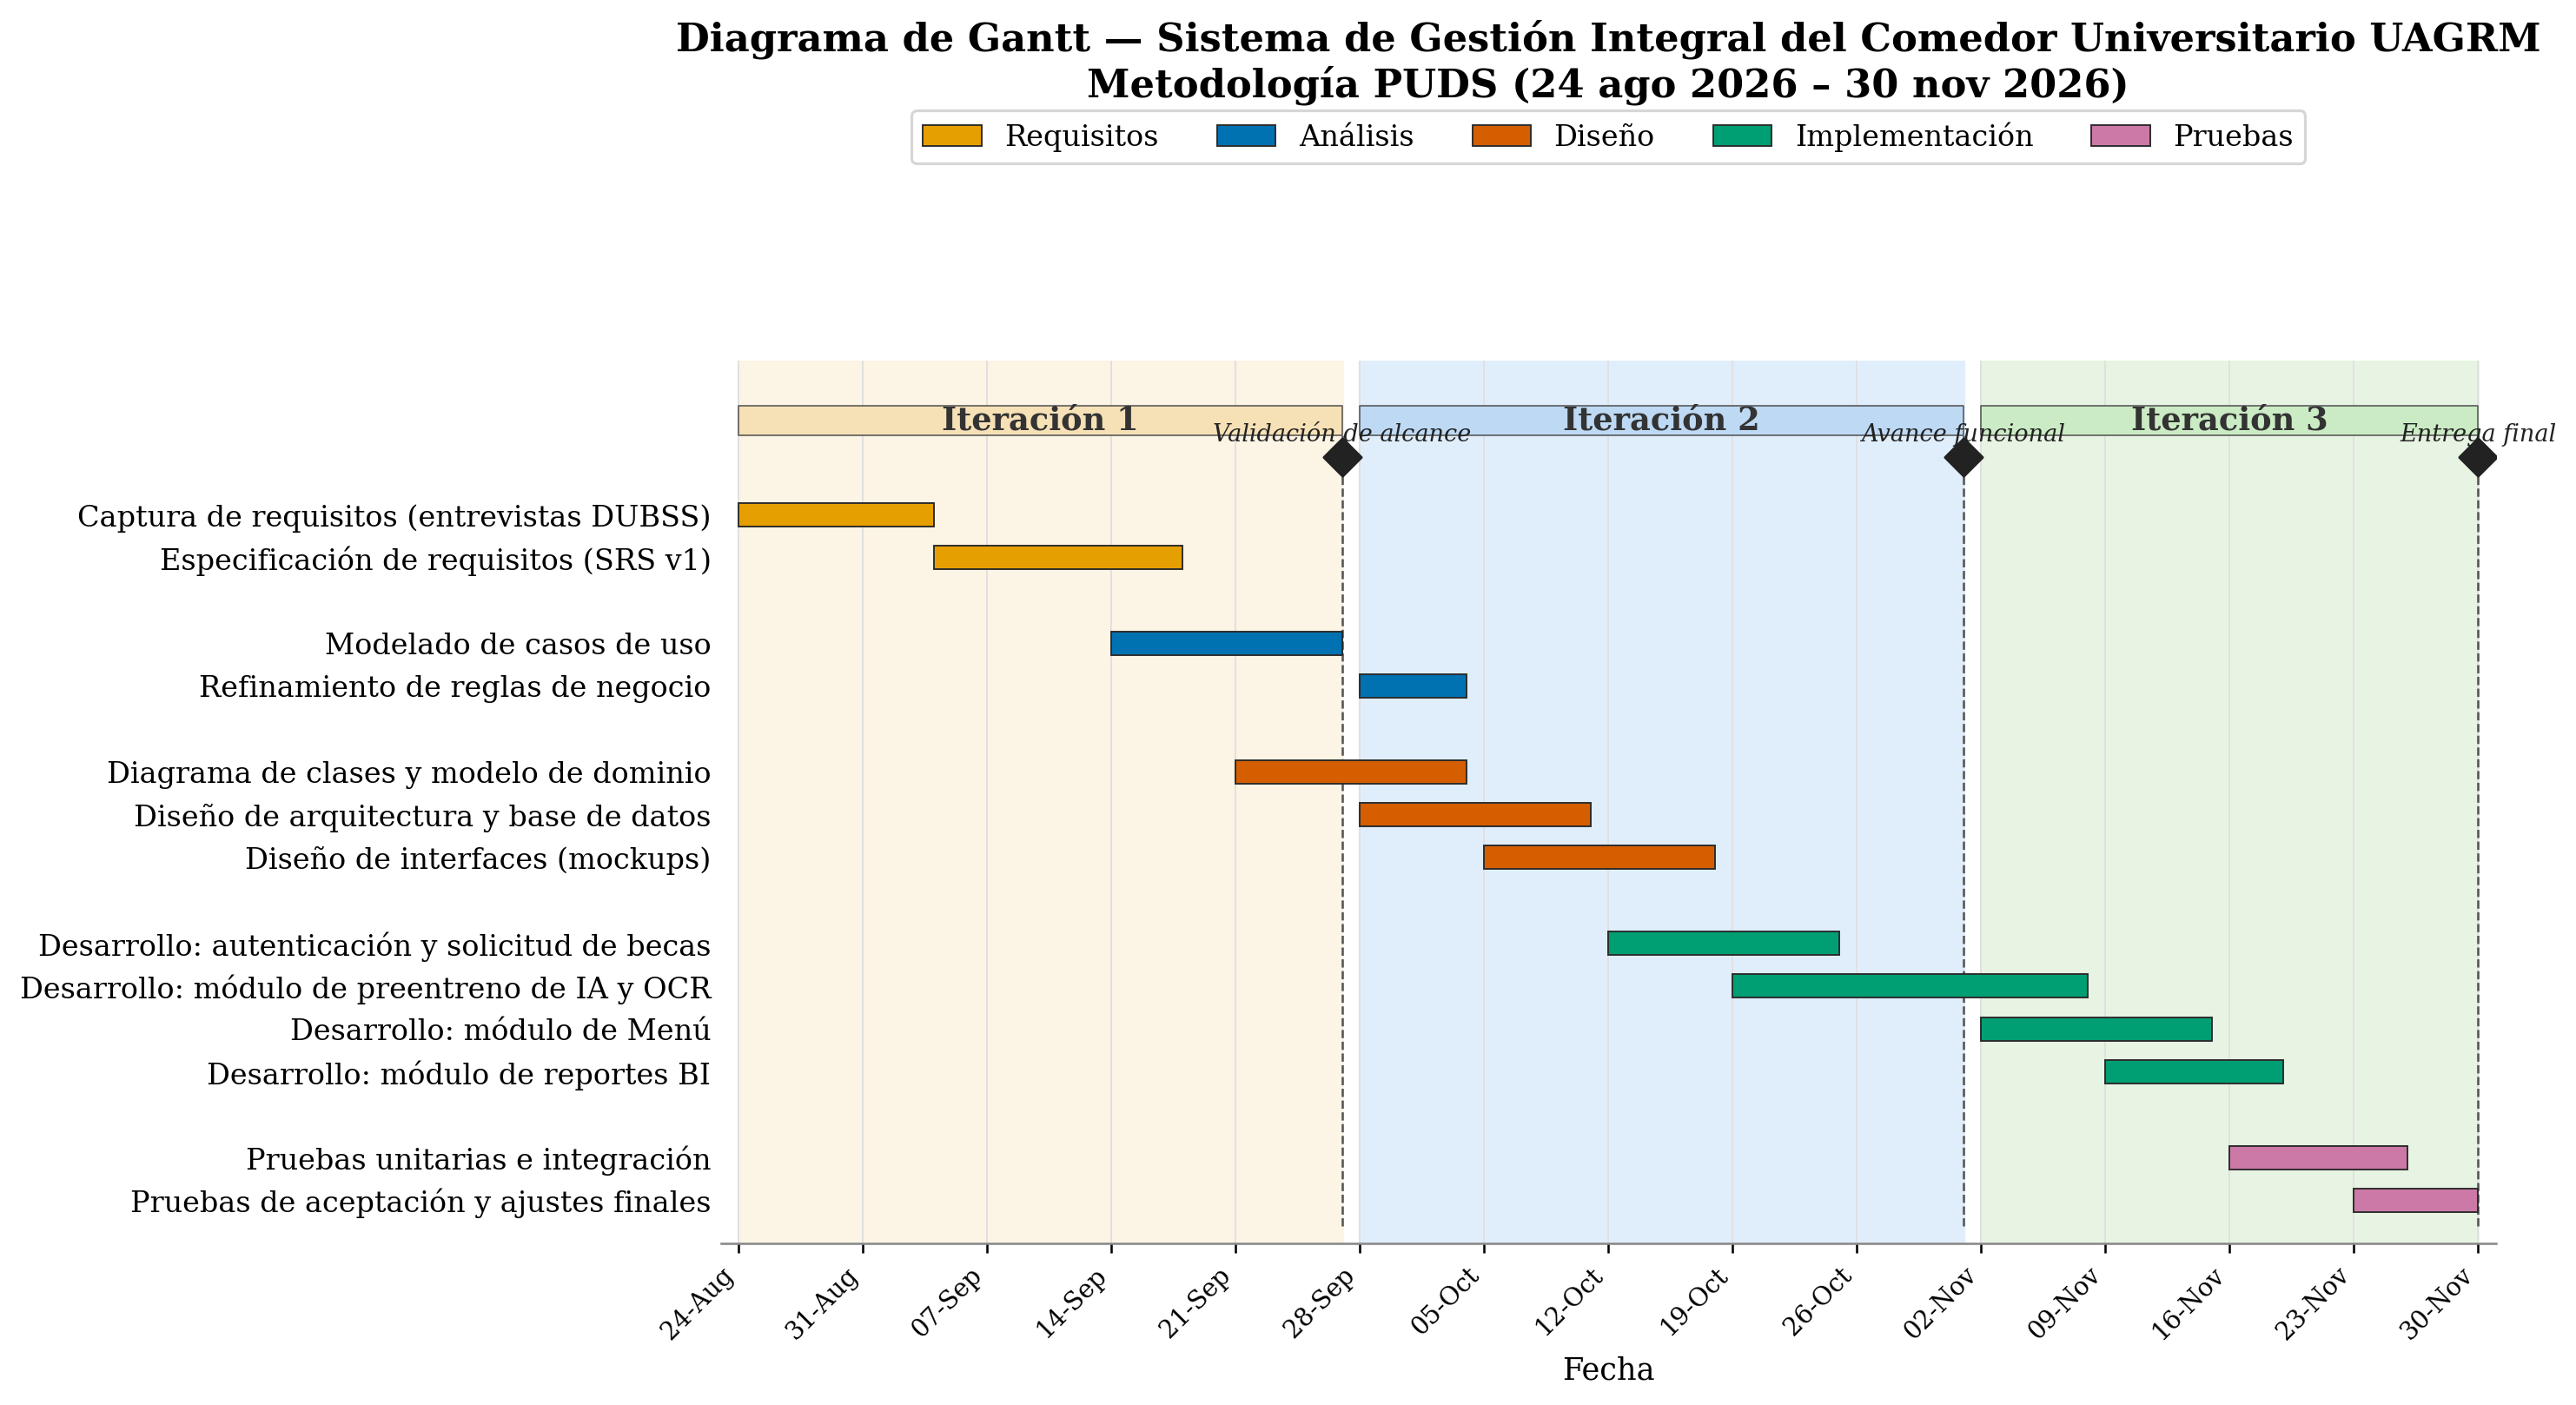
\includegraphics[width=\textwidth]{images/004_Cronograma_Gantt.png}
\smallskip
\noindent\raggedright\textit{Nota.} Elaboración propia. El diagrama detalla las fases del proyecto, sus duraciones estimadas en días hábiles y los hitos de validación de alcance, avance funcional y entrega final.
\end{figure}


% ==============================================================================
% 1.9 a 1.12: ORGANIZACIÓN, SEGUIMIENTO, TECNOLOGÍAS Y ANEXOS
% ==============================================================================
\subsection{1.9. Organización interna}

% [PENDIENTE]: Redactar "Organización interna" (equipo de 2 integrantes; confirmar tipo de organización con el equipo).

\subsection{1.10. Mecanismos de seguimiento y control}

% [PENDIENTE]: Redactar "Mecanismos de seguimiento y control" (formularios de reporte de tareas finalizadas, en proceso y de errores; confirmar con el equipo).

\subsection{1.11. Tecnologías para el desarrollo de proyecto}

Las tecnologías seleccionadas para el desarrollo se describen en el Capítulo 6 (Infraestructura para la Producción de Software); las herramientas y el hardware del equipo figuran en la sección 1.7 de este capítulo.

\subsection{1.12. Anexos}

\subsubsection{1.12.1. Líneas de código de Software de referencia 1}

% [PENDIENTE]: Salida de cloc del software 1 (ver 1.4.1.3).

\subsubsection{1.12.2. Líneas de código de Software de referencia 2}

% [PENDIENTE]: Salida de cloc del software 2 (ver 1.4.2.3).

\subsubsection{1.12.3. Líneas de código de Software de referencia 3}

% [PENDIENTE]: Salida de cloc del software 3 (ver 1.4.3.3).

